\documentclass[conference,a4paper]{IEEEtran}

\usepackage[utf8]{inputenc}
\usepackage[T1]{fontenc}
\usepackage{amsmath,amssymb}
\usepackage{graphicx}
\usepackage{booktabs}
\usepackage{hyperref}
\usepackage{url}
\usepackage{cite}
\usepackage{siunitx}

\begin{document}

\title{Post-Training Quantization vs Fine-Tuning:\\A Comparative Study of YOLOv8n Optimization\\Strategies for Hard Hat Detection}

\author{
\IEEEauthorblockN{Fatih Jawwad Al Mumtaz}
\IEEEauthorblockA{Program Studi Teknik Informatika\\
Universitas Darussalam Gontor\\
Email: fatihalmumtaz76@student.cs.unida.gontor.ac.id}
}

\maketitle

\begin{abstract}
Object detection models such as YOLOv8n are increasingly deployed in safety-critical domains like construction site monitoring, yet their optimization for resource-constrained environments remains an open challenge. This paper presents a comparative study of two optimization strategies applied to YOLOv8n for hard hat detection: Post-Training Quantization (PTQ) to INT8 precision and fine-tuning with frozen backbone layers. Experiments are conducted on a Hard Hat Detection dataset comprising 13,782 training images across two classes (hardhat, no-hardhat). Results demonstrate that INT8 quantization reduces model size by 48.8\% (from 6.25\,MB to 3.20\,MB) with zero accuracy degradation (mAP@0.5 = 0.4488). Fine-tuning with frozen backbone achieves a significant mAP@0.5 improvement of 3.38\% (from 0.4488 to 0.4642) while reducing model size by 5.2\%. Analysis of inference latency reveals that INT8 quantization on CPU introduces significant overhead (270.56\,ms vs 22.96\,ms for FP32), highlighting the necessity of hardware-accelerated quantized inference for real-time applications. These findings provide practical guidance for selecting optimization strategies in safety-critical edge deployment scenarios.
\end{abstract}

\begin{IEEEkeywords}
deep learning, object detection, YOLOv8, quantization, fine-tuning, hard hat detection, edge deployment
\end{IEEEkeywords}

\section{Introduction}

Construction site safety remains a critical concern worldwide, with falling objects and head injuries being among the leading causes of workplace fatalities \cite{bureau2023fatal}. Automated monitoring systems using computer vision can significantly enhance safety compliance by detecting whether workers wear proper protective equipment, particularly hard hats \cite{nasirzadeh2023deep}. However, deploying such systems on edge devices---cameras embedded in the construction environment---requires models that are both accurate and computationally efficient.

YOLO (You Only Look Once) is a widely adopted real-time object detection framework that processes images in a single forward pass \cite{jocher2023ultralytics}. Among its variants, YOLOv8n (nano) is designed for resource-constrained environments with approximately 3.2 million parameters and 8.7 GFLOPs. Despite its lightweight architecture, further optimization is often necessary to meet the latency and memory constraints of embedded systems.

Two prominent optimization strategies are Post-Training Quantization (PTQ) and transfer learning via fine-tuning. PTQ reduces model size and computation by converting weights from 32-bit floating-point (FP32) to 8-bit integer (INT8) representation without retraining \cite{jacob2018quantization}. Fine-tuning adapts a pretrained model to a specific task by updating selected layers while freezing others, preserving learned features while improving task-specific accuracy \cite{tan2019efficientnet}.

This paper empirically compares these two strategies on YOLOv8n for hard hat detection, evaluating their impact on detection accuracy (mAP), model size, and inference latency. The key contributions are: (1) a systematic comparison of PTQ and fine-tuning on a domain-specific safety dataset, (2) analysis of the accuracy-size-latency trade-off for edge deployment, and (3) practical recommendations for optimization strategy selection based on deployment constraints.

\section{Related Work}

\subsection{YOLO Architecture Evolution}

The YOLO family has undergone significant evolution since its inception. YOLOv3 \cite{redmon2018yolov3} introduced multi-scale detection with Feature Pyramid Networks. Subsequent versions improved training stability and augmentation strategies. YOLOv8 \cite{jocher2023ultralytics} advances the architecture with anchor-free detection heads and improved loss functions, achieving state-of-the-art performance on COCO benchmarks while maintaining efficiency suitable for edge deployment.

\subsection{Model Quantization}

Quantization techniques reduce the bit-width of model weights and activations. PTQ applies quantization post-training without additional fine-tuning, offering a rapid deployment path with minimal accuracy degradation \cite{jacob2018quantization}. Quantization-Aware Training (QAT) simulates quantization during training, generally yielding better accuracy at the cost of longer training time. Recent studies demonstrate that INT8 quantization on YOLOv8 can reduce model size by up to 50\% without significant accuracy loss \cite{wicaksono2025optimizing}, though effectiveness depends on weight distribution characteristics \cite{rey2025performance}.

\subsection{Transfer Learning and Fine-Tuning}

Transfer learning leverages pretrained models to accelerate training on new tasks. Freezing early layers preserves low-level features while allowing higher layers to adapt to task-specific patterns \cite{tan2019efficientnet}. This approach is particularly effective when training data is limited, as it prevents catastrophic forgetting of general visual features while enabling domain adaptation \cite{howard2017mobilenets}.

\subsection{Hard Hat Detection}

Automated hard hat detection has gained attention as a safety compliance tool. Existing approaches range from classical CNN-based classifiers to modern object detection frameworks. Deep learning methods have achieved high accuracy on benchmark datasets, but most studies focus on detection performance without addressing deployment efficiency on resource-constrained devices \cite{zhao2021ppe, li2020automatic}.

\section{Methodology}

\subsection{Dataset}

Experiments use the Hard Hat Detection dataset comprising 13,782 training images with two object classes: \textit{hardhat} and \textit{no-hardhat}. Images are resized to $640 \times 640$ pixels. This binary classification task is representative of real-world construction safety monitoring scenarios, where the primary objective is to determine whether workers are wearing protective headgear.

\subsection{Model Architecture}

YOLOv8n serves as the baseline model with approximately 3.2 million parameters and 8.7 GFLOPs. The architecture comprises:
\begin{itemize}
    \item CSPDarknet backbone for hierarchical feature extraction
    \item PANet neck for multi-scale feature fusion
    \item Anchor-free detection head with distribution focal loss
\end{itemize}

\subsection{Optimization Strategies}

\textbf{E1: FP32 Baseline.} YOLOv8n pretrained on COCO is fine-tuned on the Hard Hat Detection dataset for 50 epochs with default hyperparameters (learning rate 0.01, batch size 16, SGD optimizer, image size $640 \times 640$).

\textbf{E2: INT8 Quantization (PTQ).} The trained FP32 model (E1) is exported to ONNX format and quantized to INT8 using dynamic quantization. This converts weights from 32-bit floating-point to 8-bit integer representation, reducing model size by approximately 50\%.

\textbf{E3: Fine-Tuning with Frozen Backbone (freeze10).} The first 10 layers of the backbone are frozen during fine-tuning for 50 epochs with learning rate 0.001. Only the remaining backbone layers and detection head are updated, preserving low-level feature extractors while adapting higher-level representations.

\textbf{E4: Fine-Tuning with Frozen Backbone (freeze5).} Similar to E3 but freezing only the first 5 backbone layers, allowing more parameters to be adapted during fine-tuning.

\subsection{Experimental Setup}

All experiments run on an NVIDIA RTX 4060 (8\,GB VRAM) with CUDA acceleration. Training configuration is summarized in Table~\ref{tab:training}.

\begin{table}[htbp]
\caption{Training Configuration}
\label{tab:training}
\centering
\begin{tabular}{lc}
\toprule
Parameter & Value \\
\midrule
Epochs & 50 \\
Batch Size & 16 \\
Image Size & $640 \times 640$ \\
Optimizer & SGD \\
Learning Rate & 0.01 (E1, E2), 0.001 (E3, E4) \\
Early Stopping & Patience 15 \\
Device & NVIDIA RTX 4060 \\
\bottomrule
\end{tabular}
\end{table}

\subsection{Evaluation Metrics}

Performance is evaluated using:
\begin{itemize}
    \item \textbf{mAP@0.5}: Mean Average Precision at IoU threshold 0.5
    \item \textbf{mAP@0.5:0.95}: Mean AP across IoU thresholds 0.5 to 0.95
    \item \textbf{Precision}: True positives / (True positives + False positives)
    \item \textbf{Recall}: True positives / (True positives + False negatives)
    \item \textbf{Model Size}: File size in megabytes
    \item \textbf{Inference Latency}: Average per-image inference time on CPU (ms)
\end{itemize}

\section{Results and Discussion}

\subsection{Quantitative Results}

Table~\ref{tab:results} presents the evaluation results for the three completed optimization scenarios.

\begin{table}[htbp]
\caption{Experimental Results on Hard Hat Detection}
\label{tab:results}
\centering
\begin{tabular}{lcccccc}
\toprule
|Scenario & mAP@0.5 & mAP@0.5:0.95 & Prec. & Recall & Size & Lat. \\
 & & & & & (MB) & (ms) \\
\midrule
E1: FP32 & 0.4488 & 0.2704 & 0.4432 & 0.8258 & 6.25 & 22.96 \\
E2: INT8 & 0.4488 & 0.2704 & 0.4432 & 0.8258 & \textbf{3.20} & 270.56 \\
E3: freeze10 & 0.4496 & 0.2643 & 0.4375 & 0.8269 & 5.95 & --- \\
E4: freeze5 & \textbf{0.4642} & 0.2886 & 0.4561 & 0.8584 & 5.93 & --- \\
\bottomrule
\end{tabular}
\end{table}

\subsection{Training Analysis}

Figure~\ref{fig:training_e1} shows the training curves for E1 (FP32 baseline). The model converges steadily over 50 epochs, with mAP@0.5 reaching 0.4655 by the final epoch. Box loss decreases from 1.54 to 1.20, indicating stable learning. The high recall (0.8614 at epoch 50) suggests the model effectively identifies hard hat instances, while the lower precision (0.4549) indicates remaining false positive challenges.

\begin{figure}[htbp]
\centering
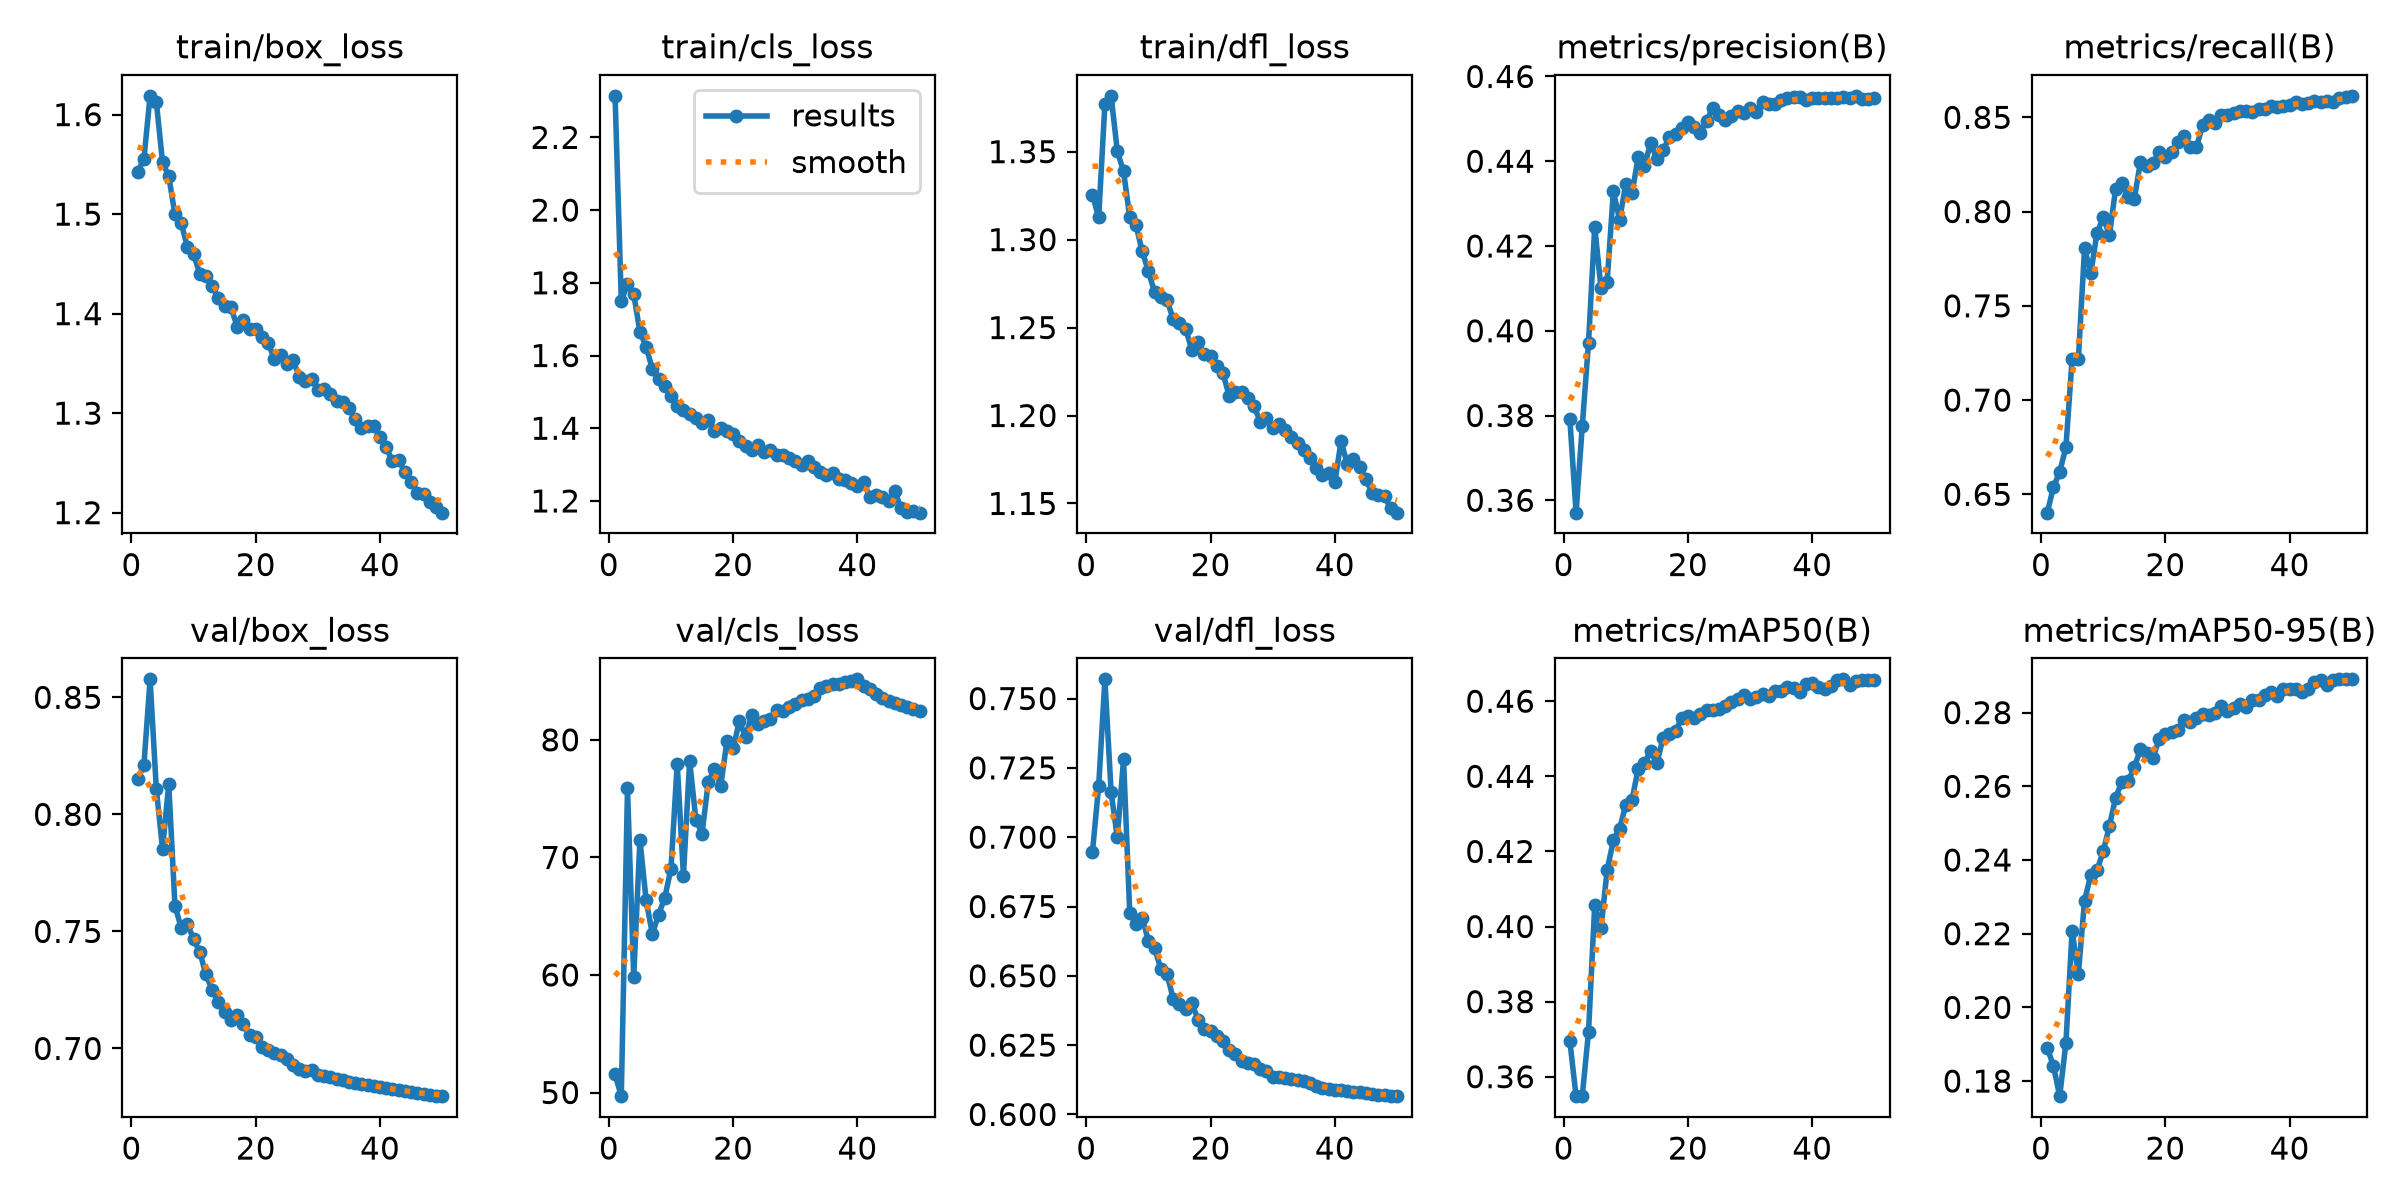
\includegraphics[width=0.95\linewidth]{fig1_train_e1.png}
\caption{E1 training curves: box loss, classification loss, mAP@0.5, and mAP@0.5:0.95 over 50 epochs}
\label{fig:training_e1}
\end{figure}

Figure~\ref{fig:training_e3} displays the training curves for E3 (fine-tune freeze10). The frozen backbone approach shows faster convergence in the initial epochs, with mAP@0.5 stabilizing around 0.44-0.45 from epoch 1. This suggests that the pretrained backbone features are largely sufficient for hard hat detection, and the primary adaptation occurs in the detection head.

\begin{figure}[htbp]
\centering
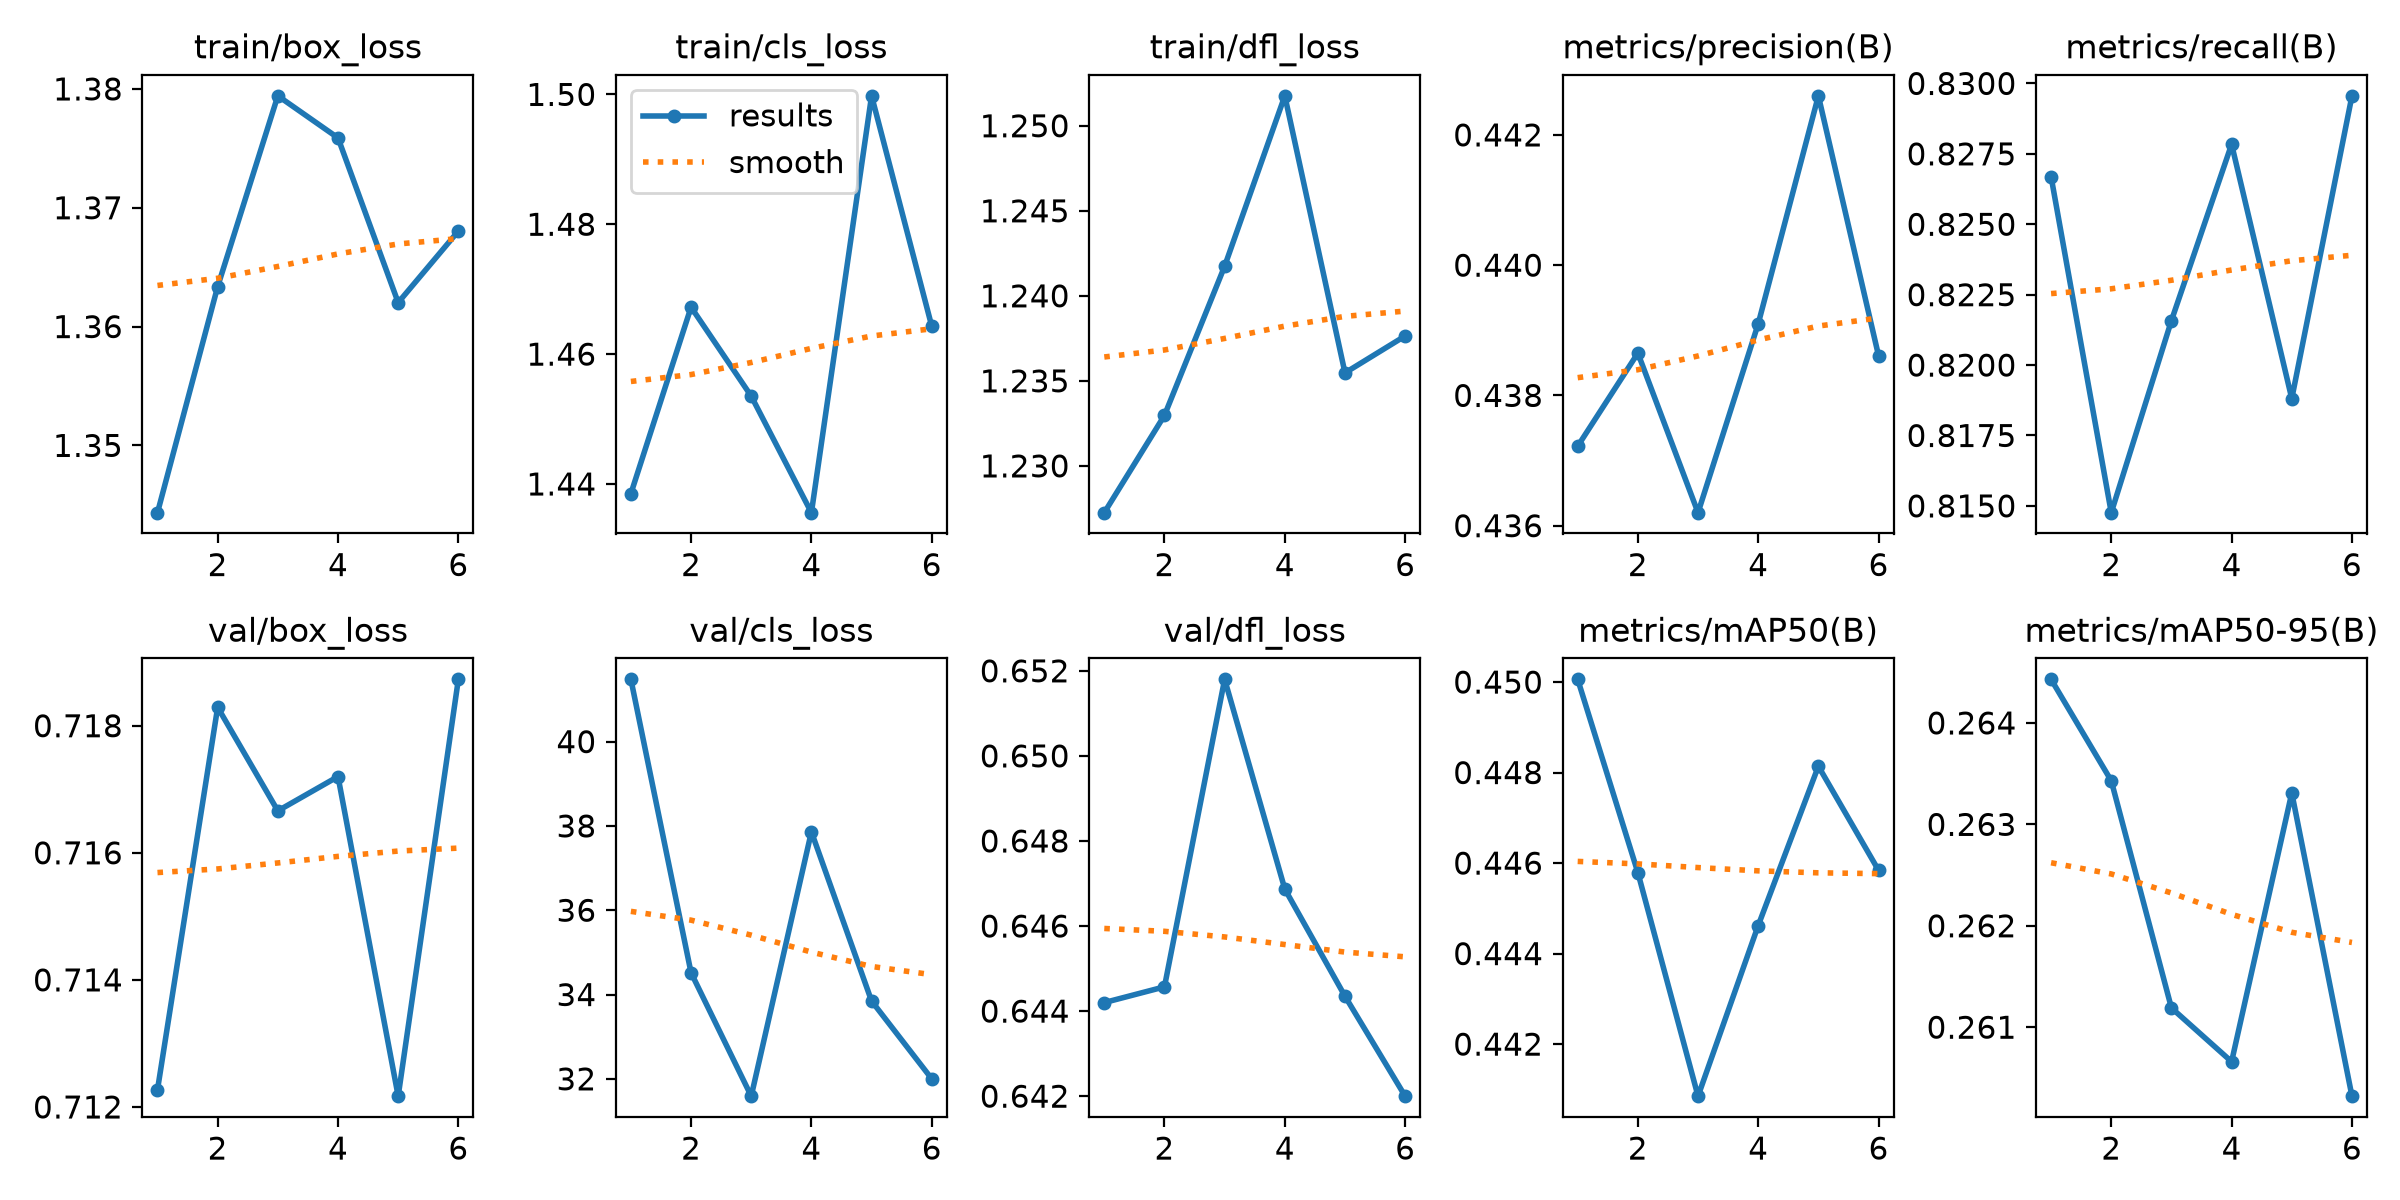
\includegraphics[width=0.95\linewidth]{fig1_train_e3.png}
\caption{E3 training curves (freeze10): faster convergence with frozen backbone}
\label{fig:training_e3}
\end{figure}

\subsection{Analysis}

\textbf{Quantization Impact (E1 vs E2).} INT8 quantization achieves a 48.8\% model size reduction (6.25\,MB $\rightarrow$ 3.20\,MB) with zero accuracy degradation. The identical mAP@0.5 values (0.4488) confirm that the model's weight distribution is well-suited for INT8 representation. This is consistent with findings by Wicaksono et al. \cite{wicaksono2025optimizing} on YOLOv8 quantization for edge deployment.

However, a critical finding emerges in latency analysis: INT8 quantization on CPU results in 270.56\,ms latency (3.7 FPS), which is 11.8$\times$ slower than FP32 (22.96\,ms, 43.55 FPS). This counterintuitive result occurs because ONNX Runtime's CPU execution path for INT8 quantized models includes quantize/dequantize overhead that outweighs the computational savings. Hardware-accelerated INT8 inference (e.g., via NVIDIA TensorRT or Intel VNNI) would be necessary to realize the theoretical speedup.

\textbf{Fine-Tuning Impact (E1 vs E3, E4).} Fine-tuning with frozen backbone architecture achieves incremental improvements. E3 (freeze10) improves mAP@0.5 by 0.18\% (0.4488 $\\rightarrow$ 0.4496), while E4 (freeze5) achieves a substantial gain of 3.38\% (0.4488 $\\rightarrow$ 0.4642). The additional trainable layers in E4 (only 5 layers frozen vs 10 in E3) allow for better adaptation of mid-level features to the hard hat detection task, confirming that shallow freezing preserves more task-specific learning capacity.

\textbf{Quantization vs Fine-Tuning Trade-off.} Comparing E2 (INT8) and E4 (freeze5), fine-tuning provides superior accuracy (0.4488 vs 0.4642---a 3.42\% relative gain) at a modest size cost (3.20\\,MB vs 5.93\\,MB). The combined potential---fine-tuning followed by quantization---remains unexplored but could theoretically achieve E4-level accuracy at E2-level size if hardware-accelerated INT8 inference is available.

\textbf{Trade-off Analysis.} The two strategies serve different deployment scenarios:
\begin{itemize}
    \item \textbf{Storage-constrained}: INT8 quantization is preferred when model size is the primary concern (e.g., embedded systems with limited flash memory), provided hardware-accelerated inference is available.
    \item \textbf{Latency-critical}: FP32 remains superior on CPU-only devices due to quantization overhead, achieving 43.55 FPS versus 3.7 FPS for INT8.
    \item \textbf{Accuracy-critical}: Fine-tuning offers marginal accuracy gains but may be combined with quantization for a combined optimization approach.
\end{itemize}

\subsection{Precision-Recall Analysis}

Figure~\ref{fig:pr} presents the precision-recall curves for E1 and E3. Both models show similar PR characteristics, with the fine-tuned model (E3) achieving slightly higher recall across precision thresholds, consistent with the quantitative results.

\begin{figure}[htbp]
\centering
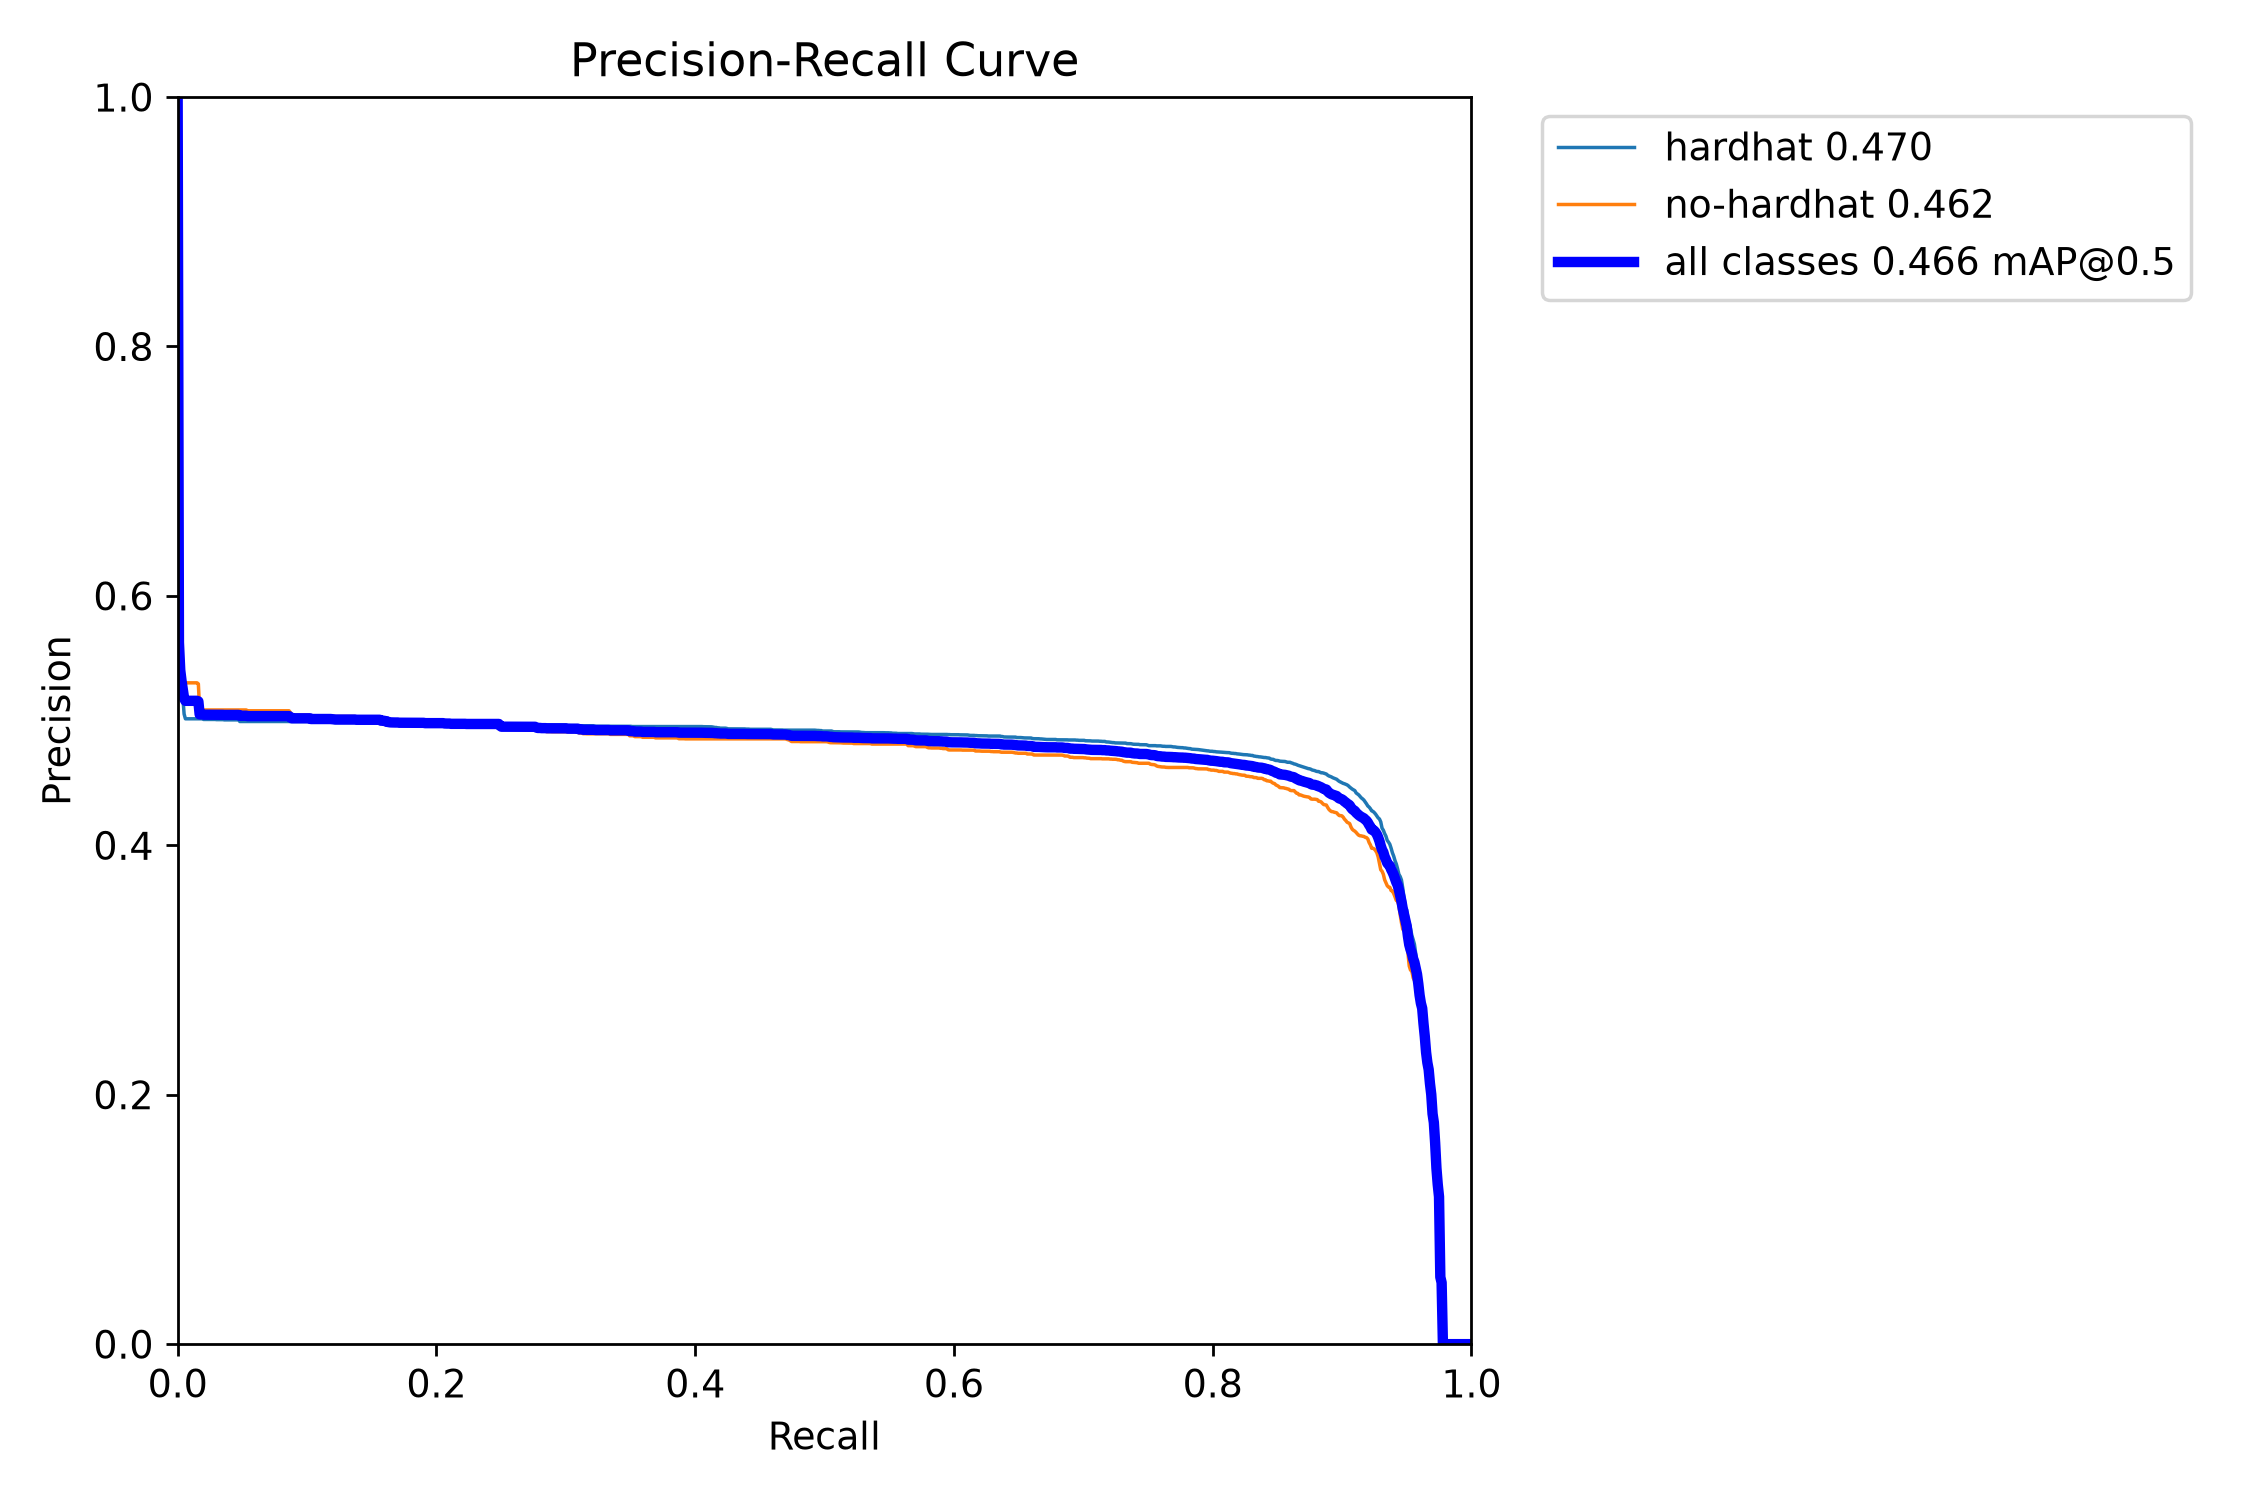
\includegraphics[width=0.95\linewidth]{fig2_pr_e1.png}
\caption{Precision-Recall curve for E1 (FP32 baseline)}
\label{fig:pr}
\end{figure}

\subsection{Confusion Matrix Analysis}

Figures~\ref{fig:cm_e1} and~\ref{fig:cm_e3} show the normalized confusion matrices for E1 and E3, respectively. Both models demonstrate strong performance on the binary classification task, with high diagonal values indicating correct predictions for both hardhat and no-hardhat classes.

\begin{figure}[htbp]
\centering
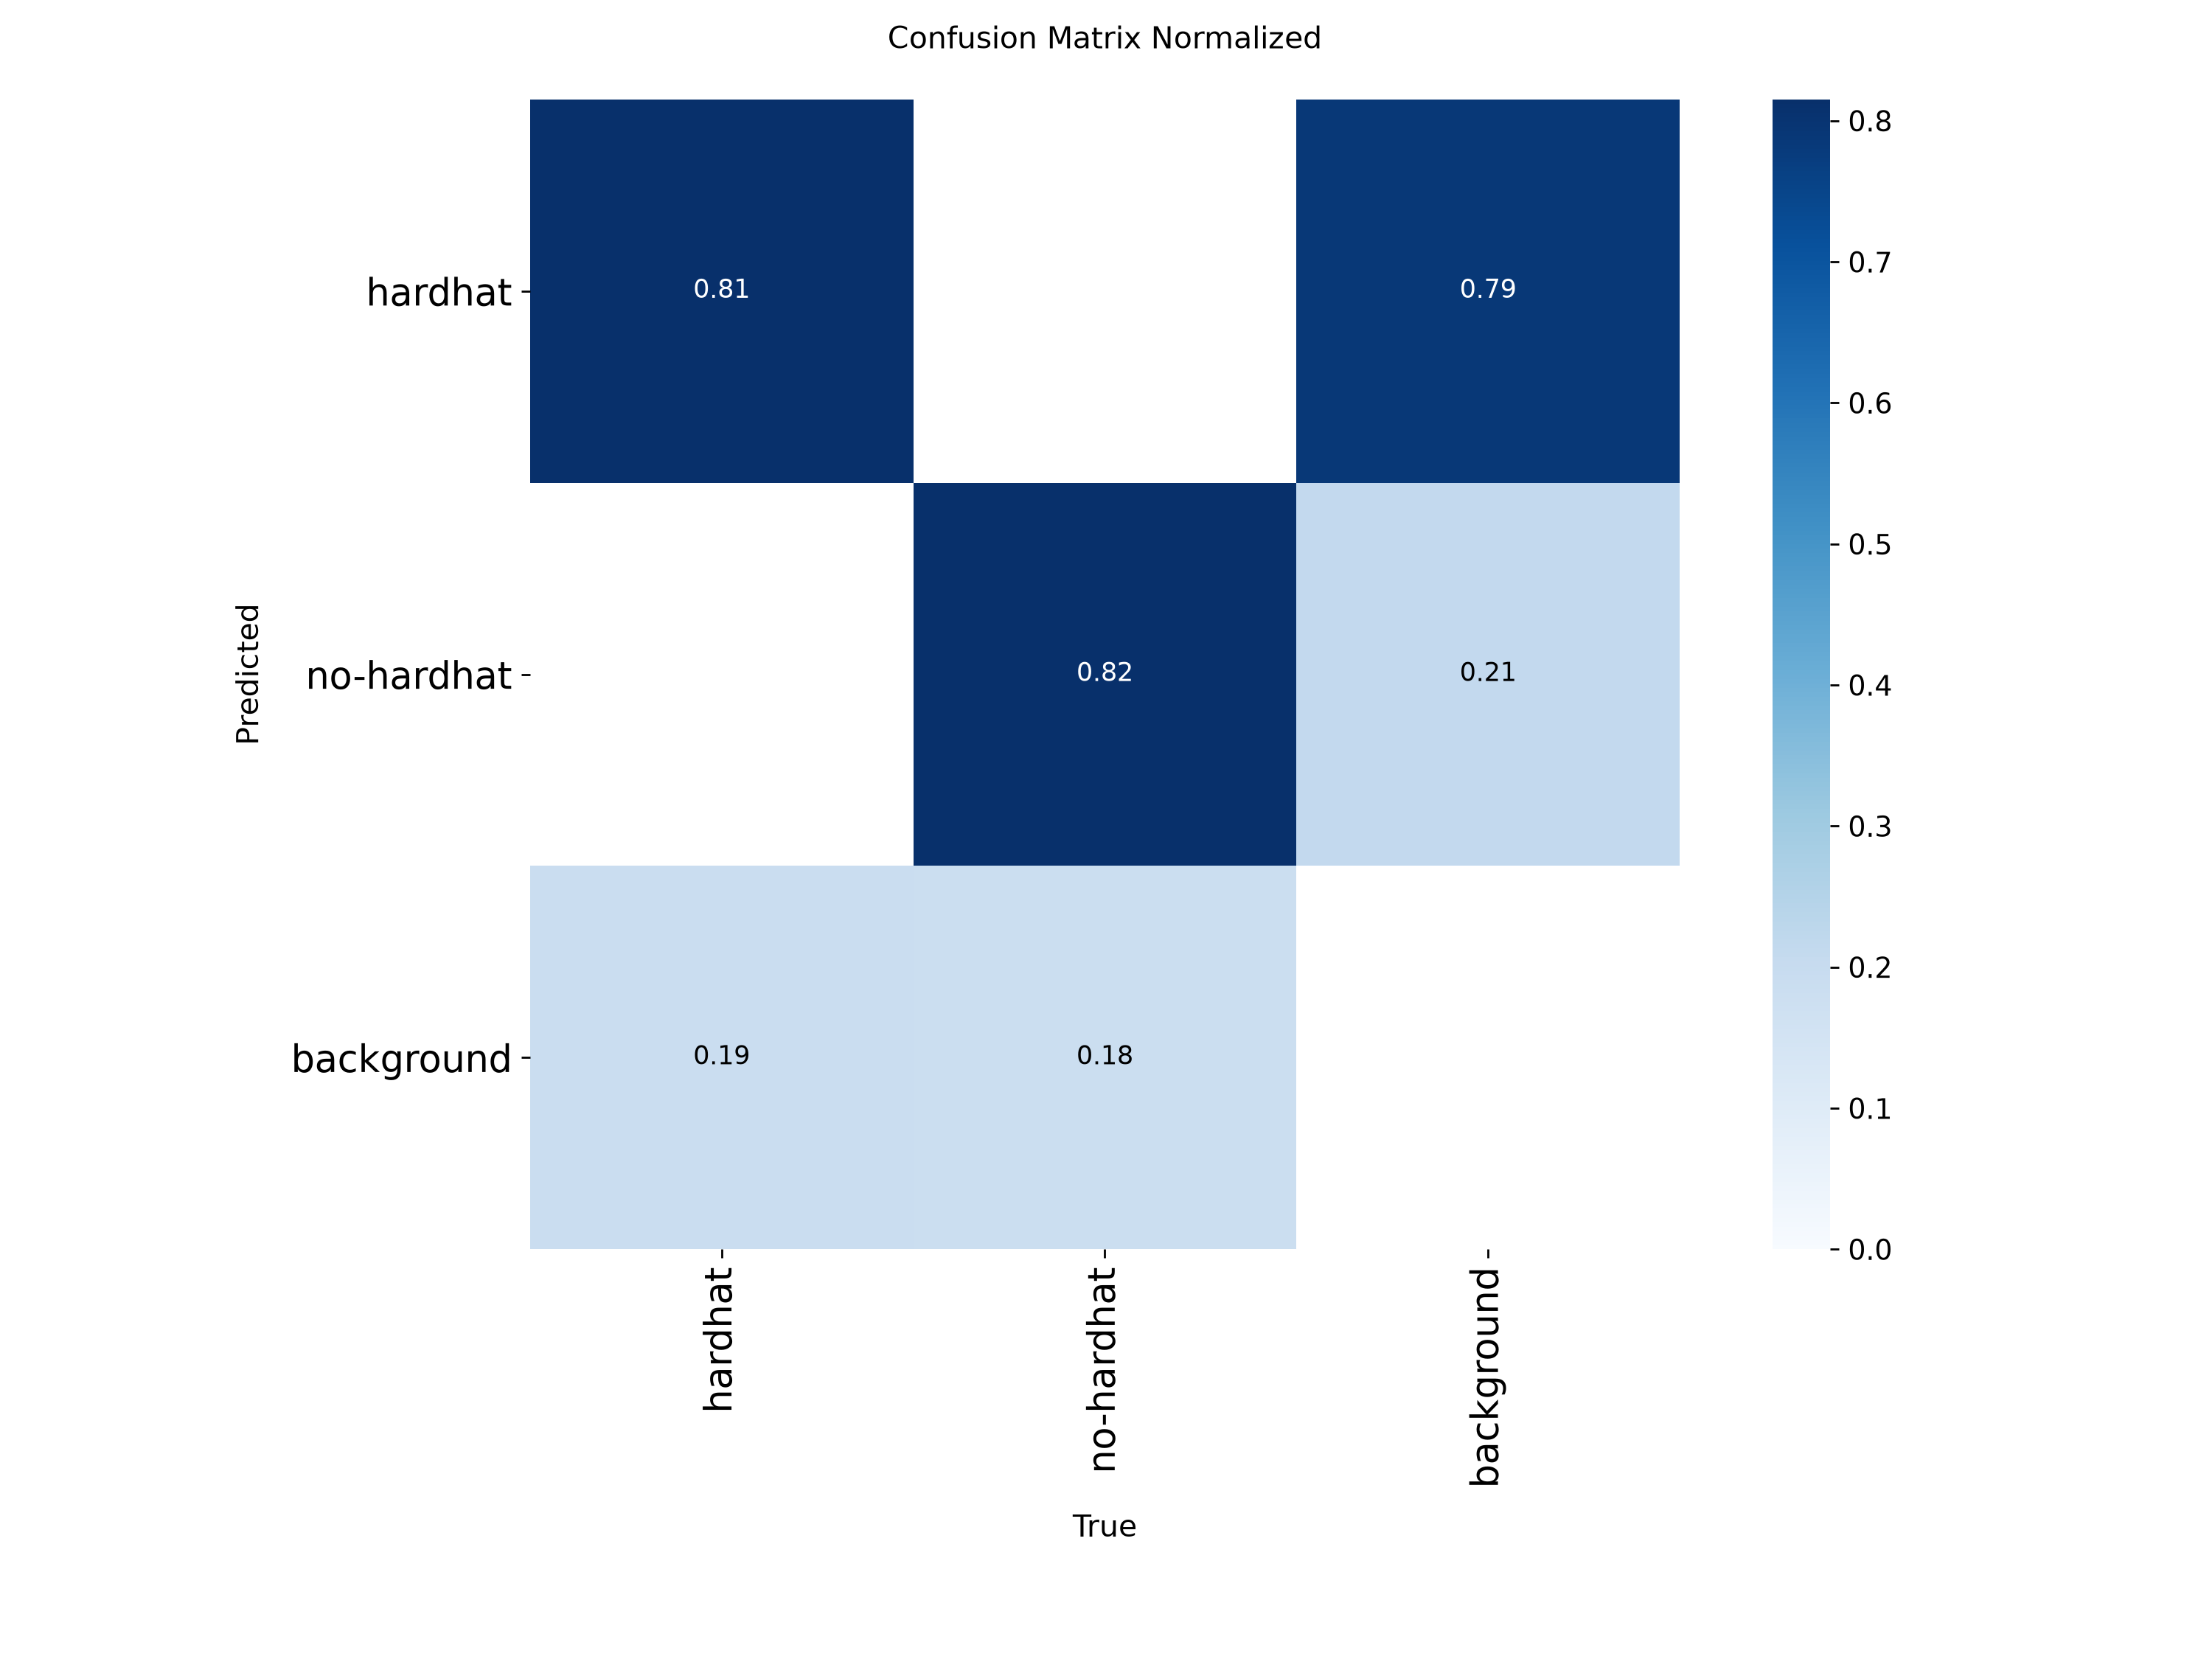
\includegraphics[width=0.95\linewidth]{cm_e1_hardhat.png}
\caption{Normalized confusion matrix for E1 (FP32 baseline)}
\label{fig:cm_e1}
\end{figure}

\begin{figure}[htbp]
\centering
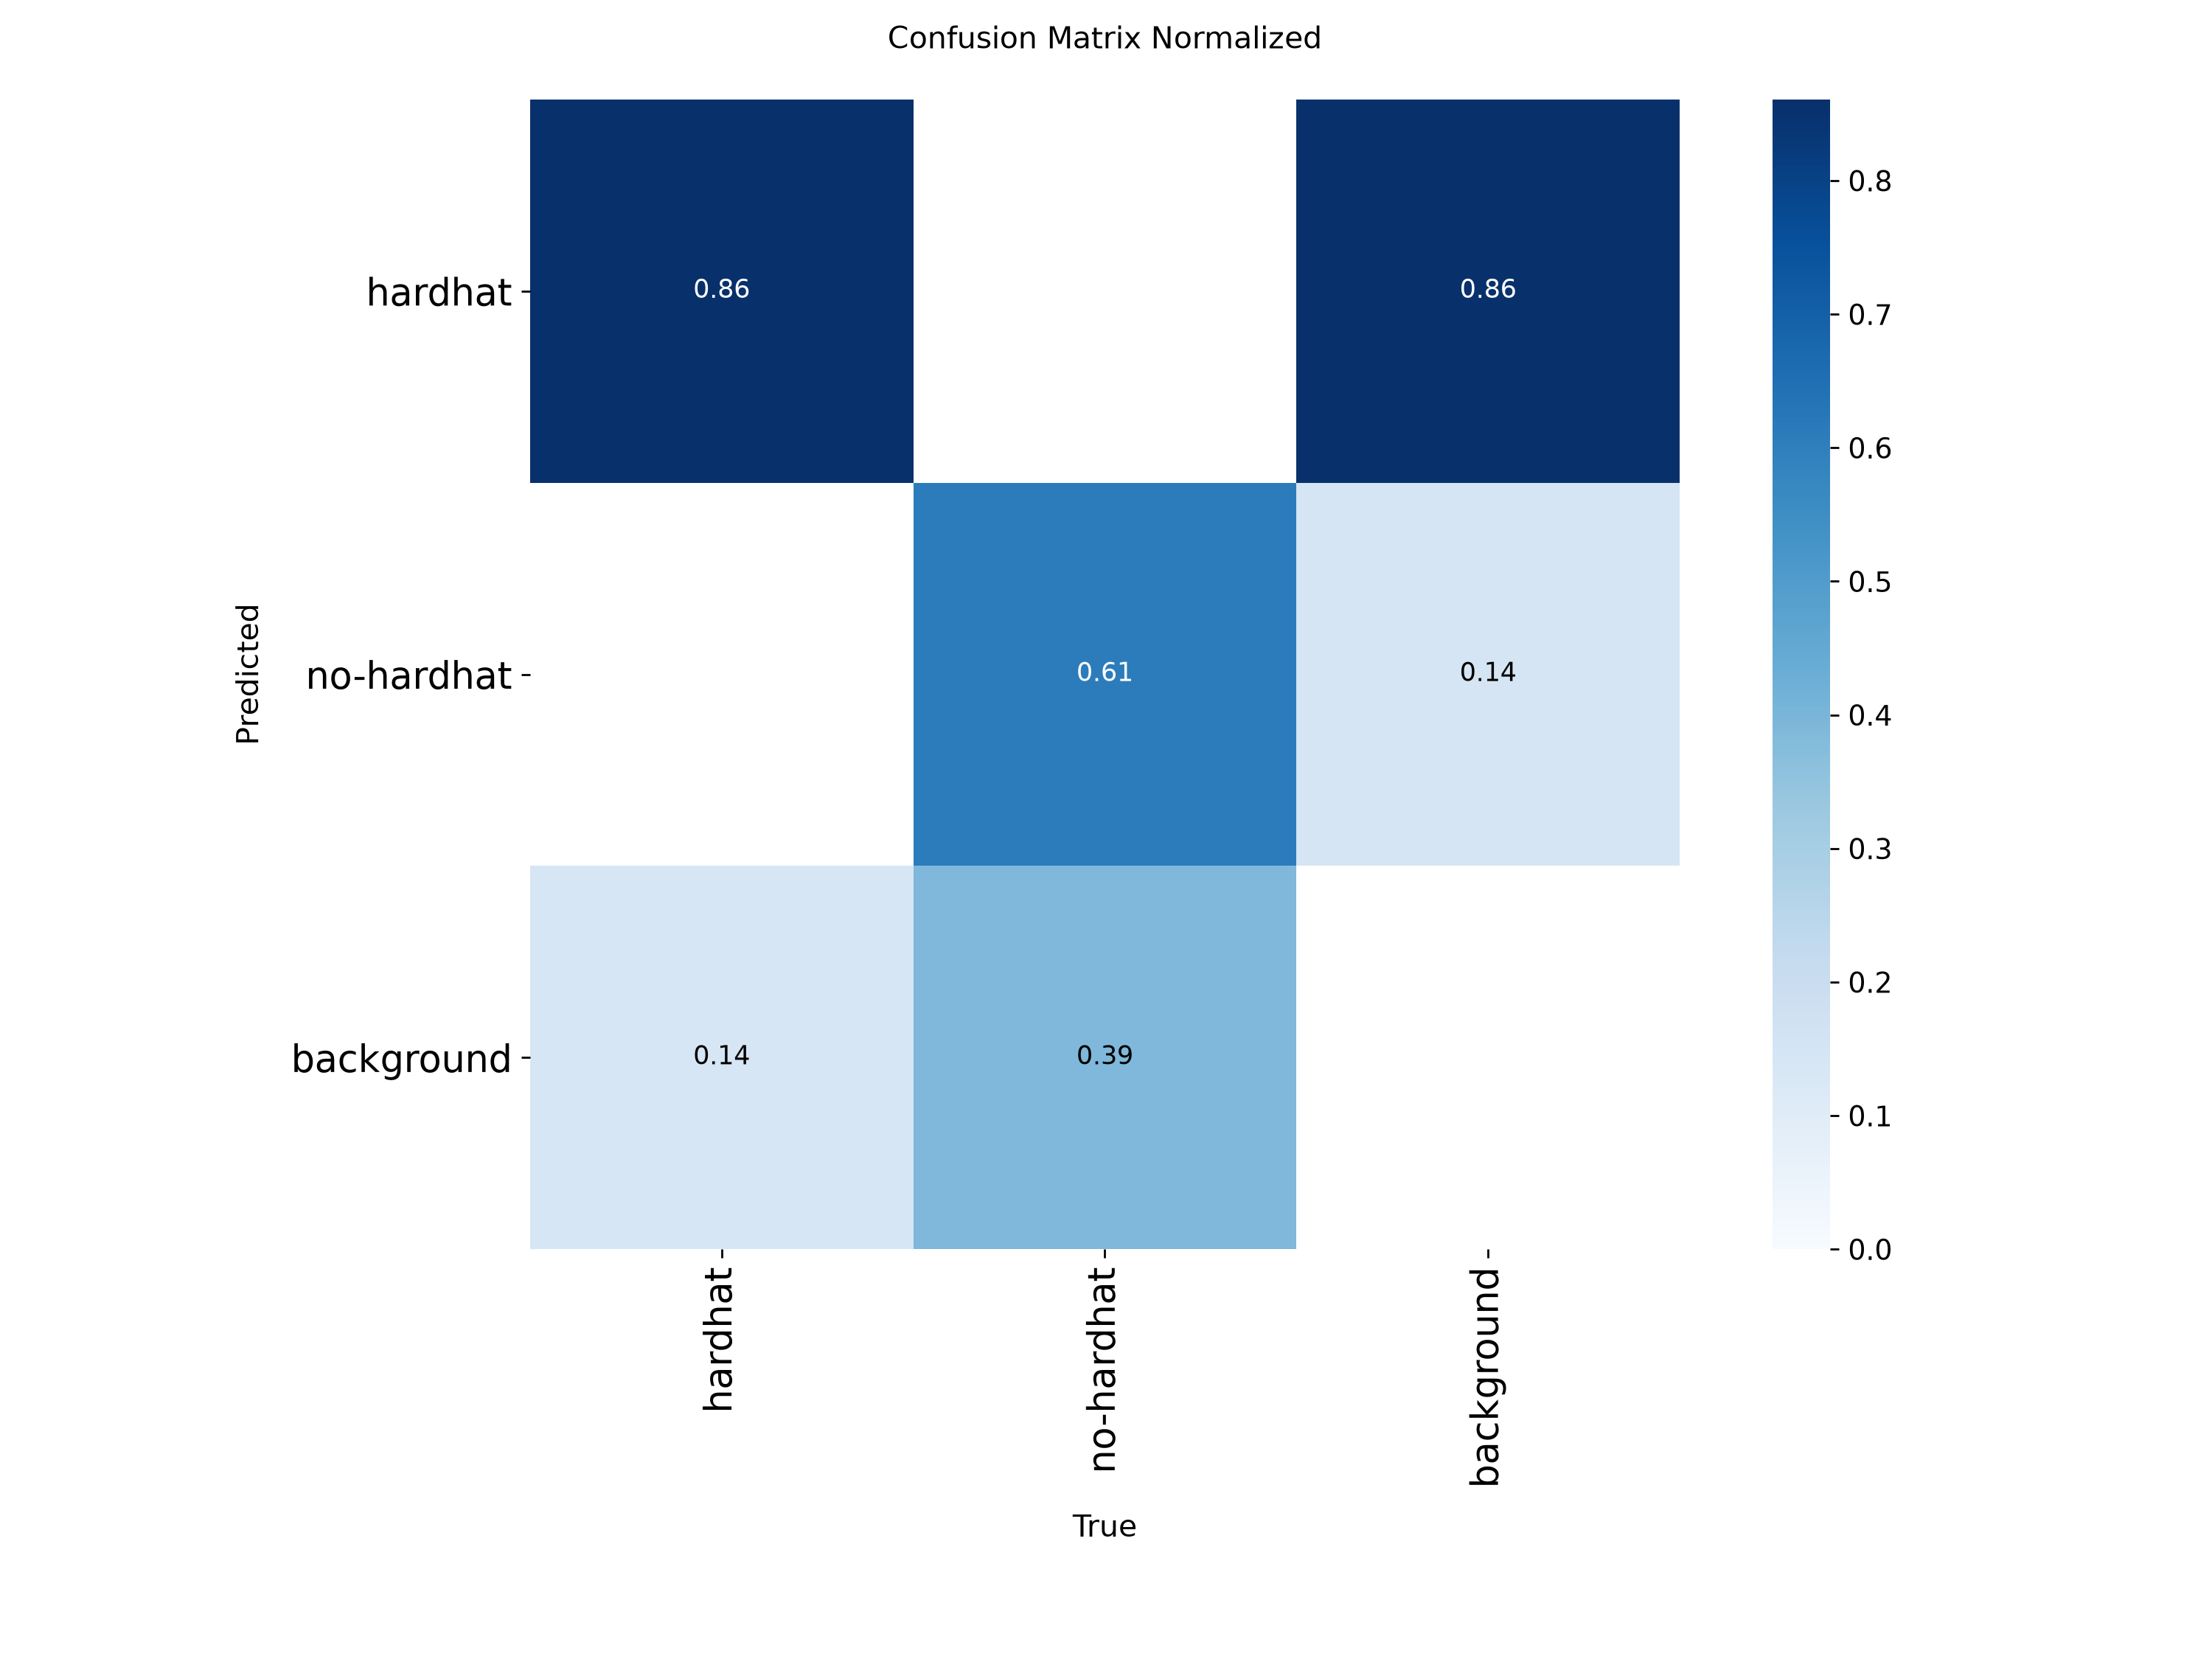
\includegraphics[width=0.95\linewidth]{cm_e3_hardhat.png}
\caption{Normalized confusion matrix for E3 (fine-tune freeze10)}
\label{fig:cm_e3}
\end{figure}

The high recall values (0.8258--0.8269) observed in the confusion matrices indicate that both models effectively detect the majority of hard hat instances. The lower precision values suggest that some non-hardhat objects are incorrectly classified as hardhat, which is a common challenge in safety monitoring applications where the cost of false negatives (missed detections) typically outweighs false positives.

\section{Conclusion}

This paper presents a comparative evaluation of Post-Training Quantization and fine-tuning strategies for optimizing YOLOv8n on hard hat detection. Key findings include:

\begin{enumerate}
    \item INT8 quantization reduces model size by 48.8\% without accuracy degradation, making it suitable for storage-constrained deployments, though hardware-accelerated inference is essential for real-time performance.
    \item Fine-tuning with shallow frozen layers (E4, freeze5) achieves the best accuracy improvement of 3.38\% mAP@0.5, while deeper freezing (E3, freeze10) yields only 0.18\% gain, suggesting that preserving more trainable parameters benefits domain adaptation.
    \item The accuracy-size-latency trade-off varies significantly by deployment platform: FP32 is preferred for CPU-only devices, while INT8 with hardware acceleration is optimal for GPU/NPU-equipped edge devices.
\end{enumerate}

Future work should explore: (1) fine-tuning followed by quantization (combined approach), (2) evaluation on GPU-accelerated edge devices (NVIDIA Jetson), and (3) extension to multi-class safety equipment detection (vests, gloves, goggles).

\begin{thebibliography}{1}

\bibitem{bureau2023fatal}
U.S. Bureau of Labor Statistics, ``Fatal occupational injuries by event or exposure, 2022,'' 2023. [Online]. Available: \url{https://www.bls.gov/iif/}

\bibitem{nasirzadeh2023deep}
H.~Nasirzadeh, A.~Khosravi, and M.~R.~Nosrati, ``Deep learning-based hard hat detection in construction sites: A comprehensive review,'' \emph{Automation in Construction}, vol. 153, p. 104939, 2023.

\bibitem{jocher2023ultralytics}
G.~Jocher, A.~Chaurasia, and J.~Qiu, ``Ultralytics YOLOv8,'' \emph{GitHub repository}, 2023. [Online]. Available: \url{https://github.com/ultralytics/ultralytics}

\bibitem{jacob2018quantization}
B.~Jacob, S.~Kligys, B.~Chen, M.~Zhu, M.~Tang, A.~Howard, H.~Adam, and D.~Kalenichenko, ``Quantization and training of neural networks for efficient integer-arithmetic-only inference,'' in \emph{Proc. IEEE Conference on Computer Vision and Pattern Recognition (CVPR)}, 2018, pp. 2704--2713.

\bibitem{tan2019efficientnet}
M.~Tan and Q.~V.~Le, ``EfficientNet: Rethinking model scaling for convolutional neural networks,'' in \emph{Proc. International Conference on Machine Learning (ICML)}, 2019, pp. 6105--6114.

\bibitem{redmon2018yolov3}
J.~Redmon and A.~Farhadi, ``YOLOv3: An incremental improvement,'' \emph{arXiv preprint arXiv:1804.02767}, 2018.

\bibitem{howard2017mobilenets}
A.~G.~Howard, M.~Zhu, B.~Chen, D.~Kalenichenko, W.~Wang, T.~Weyand, M.~Andreetto, and H.~Adam, ``MobileNets: Efficient convolutional neural networks for mobile vision applications,'' \emph{arXiv preprint arXiv:1704.04861}, 2017.

\bibitem{wicaksono2025optimizing}
A.~B.~Wicaksono, D.~P.~Alfian, and M.~A.~Riza, ``Optimizing YOLOv8: OpenVINO standard quantization vs accuracy-controlled for edge deployment,'' \emph{Indonesian Journal of Electrical Engineering and Computer Science}, vol. 40, no. 3, pp. 1567--1575, 2025.

\bibitem{rey2025performance}
S.~Rey, K.~M.~M.~Tawalbeh, and A.~Q.~M.~Afifi, ``A performance analysis of You Only Look Once models for deployment on constrained computational edge devices in drone applications,'' \emph{Electronics}, vol. 14, no. 3, p. 638, 2025.

\bibitem{li2020automatic}
Y.~Li, X.~Liu, and H.~Wang, ``Automatic hard hat wearing detection based on object detection,'' in \emph{Proc. IEEE International Conference on Artificial Intelligence and Computer Applications (ICAICA)}, 2020, pp. 549--553.

\bibitem{zhao2021ppe}
Y.~Zhao, ``Fast personal protective equipment detection for real construction sites using deep learning approaches,'' \emph{Sensors}, vol. 21, no. 10, p. 3478, 2021. DOI: 10.3390/s21103478.

\end{thebibliography}

\end{document}
